\textcolor{red}{
\begin{itemize}
    \item Discuss any analysis supporting the sizing analysis.
    \item Discuss future work.
    \item AIAA: A V-n diagram for the aircraft with identification of necessary aircraft velocities and design load factors.
    Required gust loads are specified in 14 Code of Federal Regulations (CFR) Part 25. (This may not come until later)
    \item AIAA: Materials selection for main structural groups and general structural design, including layout of primary airframe structure as well as the strength capability of the structure
    and how that compares to what is required at the ultimate load limits of the aircraft.
    The maximum dive speed of the aircraft shall be specified. (this may not come until later)
\end{itemize}}

\subsection{Structures}
\subsubsection{Material Selection}
Modern-age aircraft exhibit many different structure layouts and material selection for each structure. The goal for the material selection is to meet the given requirements, as well as provide an aircraft which will have the best mechanical properties for the given flight missions. The different structure types are tabulated in Table \ref{tab:structure_material_table}.

\begin{table}[!h]
\centering
\caption{Structures Build-up Descriptions }
\label{tab:structure_material_table}
\begin{tabular}{ |p{2cm}|p{13cm}| }
\hline
\multicolumn{1}{|c|}{\textbf{Build-up Type}} & \multicolumn{1}{c|}{\textbf{Description}}                                                                                                                       \\ \hline
Metal                                        & Most or all parts apart of the primary and secondary structure are metallic, such as aluminum, steel, and titanium                                              \\ \hline
Composite                                    & Most or all parts apart of the primary and secondary structure are composite, such as carbon fiber reinforced polymers (CFRP), fiber glass, or other composites \\ \hline
Hybrid                                       & Depending on the structure, the material of the structure is either metal or composite                                                                            \\ \hline
\end{tabular}
\end{table}
% \begin{tabular}{ |p{3cm}||p{3cm}|p{3cm}|p{1.5cm}|p{3cm}| }

Metallic build-up is the more traditional method of designing aircraft structure, where most or all primary structures are composed of metal alloys. This method of construction is typically cost-effective and weight efficient for most structures, however, there are downsides such as damage tolerance and fatigue. A composite build-up required high development costs, and relatively high manufacturing costs, but can offer incredible weight-savings compared to metal structure. \textcolor{red}{Find source for density to ultimate tensile strength} A hybrid build-up is a method where both metals and composites are used for different structures depending on key factors such as fatigue, damage tolerance, ultimate strength per density ratio, cost of manufacturing, assembly methods, and operational costs. Hybrid designs usually optimized costs and weight of the structure, which results in the wings and stabilizers to be a mainly composite build-up, and the fuselage and other secondary structures are metal build-up. 

Hybrid construction is a newer technology, and as manufacturing of composites develops more, this style of construction may be used more in industry. A notable aircraft which uses a hybrid build would be the B777-X, where the wings and stabilizers are composite and the fuselage is metallic. The reason the fuselage is metallic and not composite comes down to the difficulties in manufacturing a round and continuous composite structure, such as the fuselage and empennage sections. A notable aircraft which utilizes mainly composite construction is the B787, see Fig \ref{fig:787 materials}

\begin{figure}[!h]
    \centering
    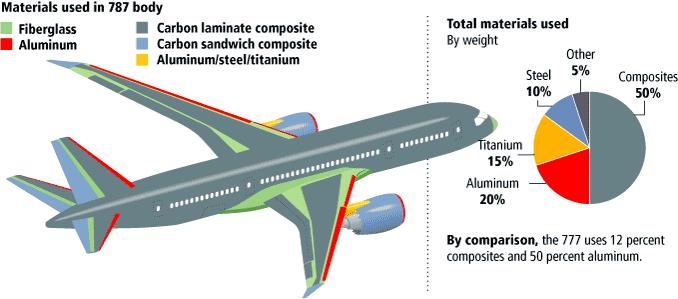
\includegraphics[width=\linewidth]{Photos/787 Materials.png}
    \caption{Material Composition of the B787}
    \label{fig:787 materials}
\end{figure}

In Table \ref{tab:structure_material_pugh}, the pros and cons for each build-up construction method were weighed in a Pugh matrix given the requirements of cost reduction and the desired aspect ratio and wingspan.

%Insert pugh matrix

Given the Pugh matrix, a hybrid construction is most ideal for the given aircraft requirements. A low fidelity analysis of the structure can assume and isotropic material with the mechanical properties of an ideal composite layup to create a factor to apply to estimations of structure loading given by Raymer (\textcolor{red}{find sources)}. A high fidelity analysis of the composite structure would require one of two methods: run FEA on an isotropic material with similar properties to an ideal composite layup, or run FEA with a specific composite build-up in a capable software such as ANSYS.

\subsubsection{Construction and Layout}
Given the hybrid construction method, the wings and stabilizers require a newer method of construction compared to the traditional metallic construction. 

Since composites are essentially created via additive manufacturing techniques, the stringers can be integral in the upper and lower panels of the wings and stabilizers. This alone saves incredible costs and weight by eliminating the use of fasteners in high-load locations. No fasteners also increases the damage tolerance and fatigue rating of the structure.

Spars are the most important structure to the wings, and arguable the most important on the entire aircraft. These few parts make the entire aircraft fly, and in the process, see a lot of loading cycles over the life of the aircraft. In metal structures, loading cycles cause fatiguing, and then fatigue cracking, which degrades the structure. Traditionally, metallic structures use a 3-piece build-up for the spar: chord on the top and bottom, and a web connecting the two chords. This structure ends-up looking like a C-channel extrusion. The reason the spars are a 3-piece build-up comes down to crack growth and fatigue. A crack starts in the lower chord, but cannot grow through the entire spar since the chord is connected to the web by fasteners. There are a few aircraft that have used a one-piece, or monolithic, metallic spar, some being the B1-B and the A320 NEO. There is significant research in learning crack-growth patterns and predicting where cracks will start and grow, which would open-up huge possibilities in reducing manufacturing costs by allowing optimized metallic spars to be utilized on low-cost aircraft.

The spars are where composites differ greatly from traditional 3-piece spar construction. Since composite structures don't crack like metal structures when fatigued, a monolithic spar can be utilized. This spar construction reduces costs, but increases the weight 


\subsection{Loads (\textit{MK})}
One important aspect in the structural analysis of the aircraft is determining the limits in the performance of the aircraft. This is specifically done using a V-N diagram, as shown in Figure \ref{figVN}. This diagram incorporates parameters such as wing loading and performance velocities (maneuvering, cruise, and dive velocities) along with limit loading factors. Maximum positive and negative limit loading factors of 3.2 and -1.5 were chosen, respectively, according to the regulations set forth in FAA 14 CFR Part 25.337, Limit Maneuvering Load Factors. These limit loading factors also contain a safety factor of 1.5, as specified in FAA 14 CFR Part 25.303, Factor of Safety. One note about the diagram is that the velocities are displayed as equivalent velocities (KEAS).

\begin{figure}[H]
    \centering
    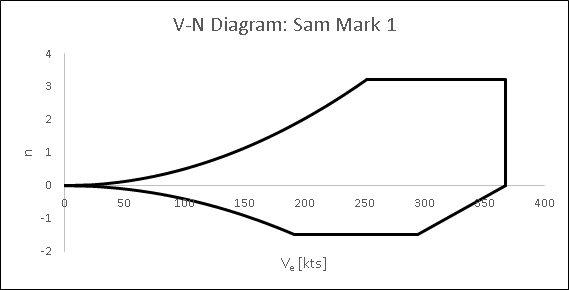
\includegraphics{Photos/VN_Diagram_(2-11-20).png}
    \caption{VN Diagram of Limit Load Factors}
    \label{figVN}
\end{figure}
